
\section{Materials and Methods}
\label{methods}

\subsection{Input Graph}

We build the network model using data provided by the Lebanese ministry of energy and water. This dataset contains information about every power plant generator (sources for power), high-to medium voltage transmission substations, medium to low voltage distribution stations that disseminate power directly to subscribers, as well as transmission lines through which power dissipates. Transmission lines exist between generators and transmission substations, as well as among transmission substations, distribution substations, and finally, between transmission and distribution substations. 


\secondedited{
The power grid consists of generating stations responsible for the power production, which is transmitted through high voltage lines to demand centers, which then, in turn, distribute power to the consumers.  This design entails the emergence of a large number of connected components which is a universal feature of grids with a characteristic power-law degree distribution~\cite{RosasCasals:2007td,Bompard:2009ga,Brummitt:2013jj,Daqing:2014bp,Albert:2004bw,Wang:2011js,Sole:2008cv}.}
%
There are five major power plants in Lebanon. Transmission and distribution substations are such that they receive power from all of the major power plants, and so, if all but one such plant is hit, the entire network can still receive power. Because of this redundancy, the only way to achieve total failure is through the obvious choice of attacking all five power plants. 
%
\edited{
To exclude this obvious scenario from our contingency analysis, the data received directly from the Lebanese ministry of power and energy does not include all five power plants from the associated graph model. This renders our contingency analysis completely focused on the irredundant nodes constituting transmission and distribution substations, where the corresponding graph representation of the power grid consists of several connected components. }
%
\secondedited{
We should note that in the original dataset these five vertices were assigned a tag which described them as redundant. Therefore no extra computational work was done to identify them. In the event that the power network fails to manifest a large number of connected components that permit for the kind of distribution we are adopting in the present manuscript, one can attempt to distribute/parallelise the low-level graph Betweenness Centrality and Single Source Shortest Paths algorithms employed, using, for example, a number of distributed and parallel tools available in~\cite{Bertolucci16,Djidev14, Edmonds10, Jin10, Kumbhare14, Redekopp13, Solomonik13}, to cite a few.}
%
Our analysis simulates attacks on both transmission as well as distribution substations. It also pursues inter-dependencies as failures propagate within a single connected component, and addresses the overall loss of connectivity to all subscribers as a result. Finally, our analysis adopts the idealised (and simplified) view that capacity across the transmission lines is never jeopardised, and thus failure of the network is a result of attacks on substations only.

Our resulting network model consists of an undirected, unweighted graph with $679965$ edges, representing transmission/distribution lines, and $899162$ vertices, representing transmission/distribution substations. This is one order of magnitude larger than the graph treated in \cite{2000Natur.406..378A}, and is a consequence of the fact that the given Lebanese power grid representation captures extremely fine grained spatial coordinates, yielding all distribution substations no matter how minor. Our distribution analysis of the degrees of vertices confirms that indeed, the resulting graph exhibits a power law distribution (Fig. \ref{fig:degree-vertices}). 
%Also, our analysis is holistic in the sense that it simulates attacks on both transmission as well as distribution substations. 
%insert figure here

\begin{figure}[!tbp]
  \centering
     {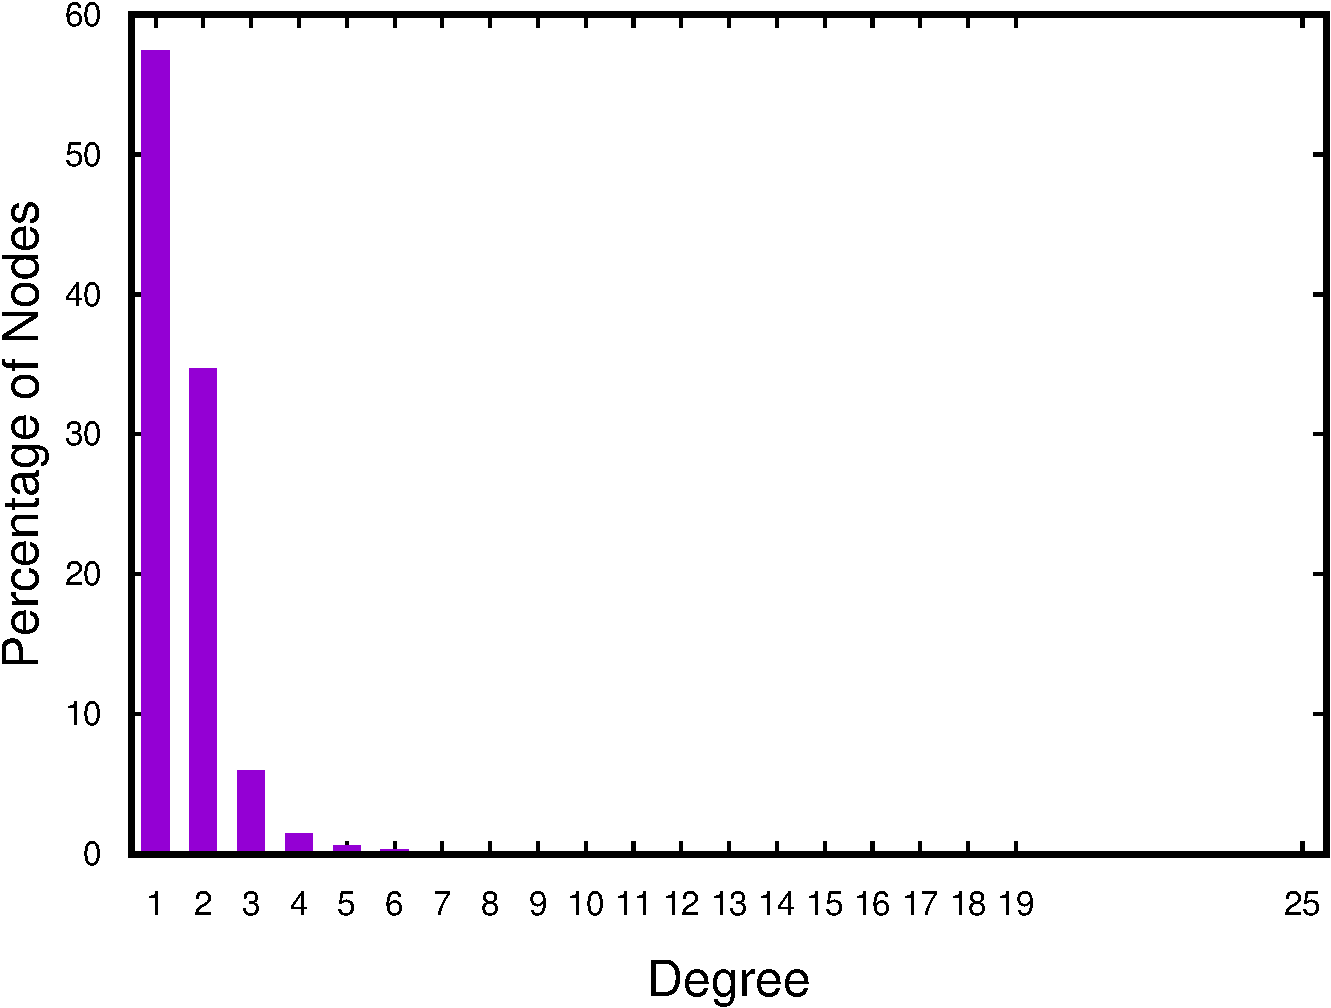
\includegraphics[scale=0.35]{bench/generated/degree-counter-crop.pdf}}
  \caption{Degree of vertices}
    \label{fig:degree-vertices}
\end{figure}

\begin{figure}
\centering
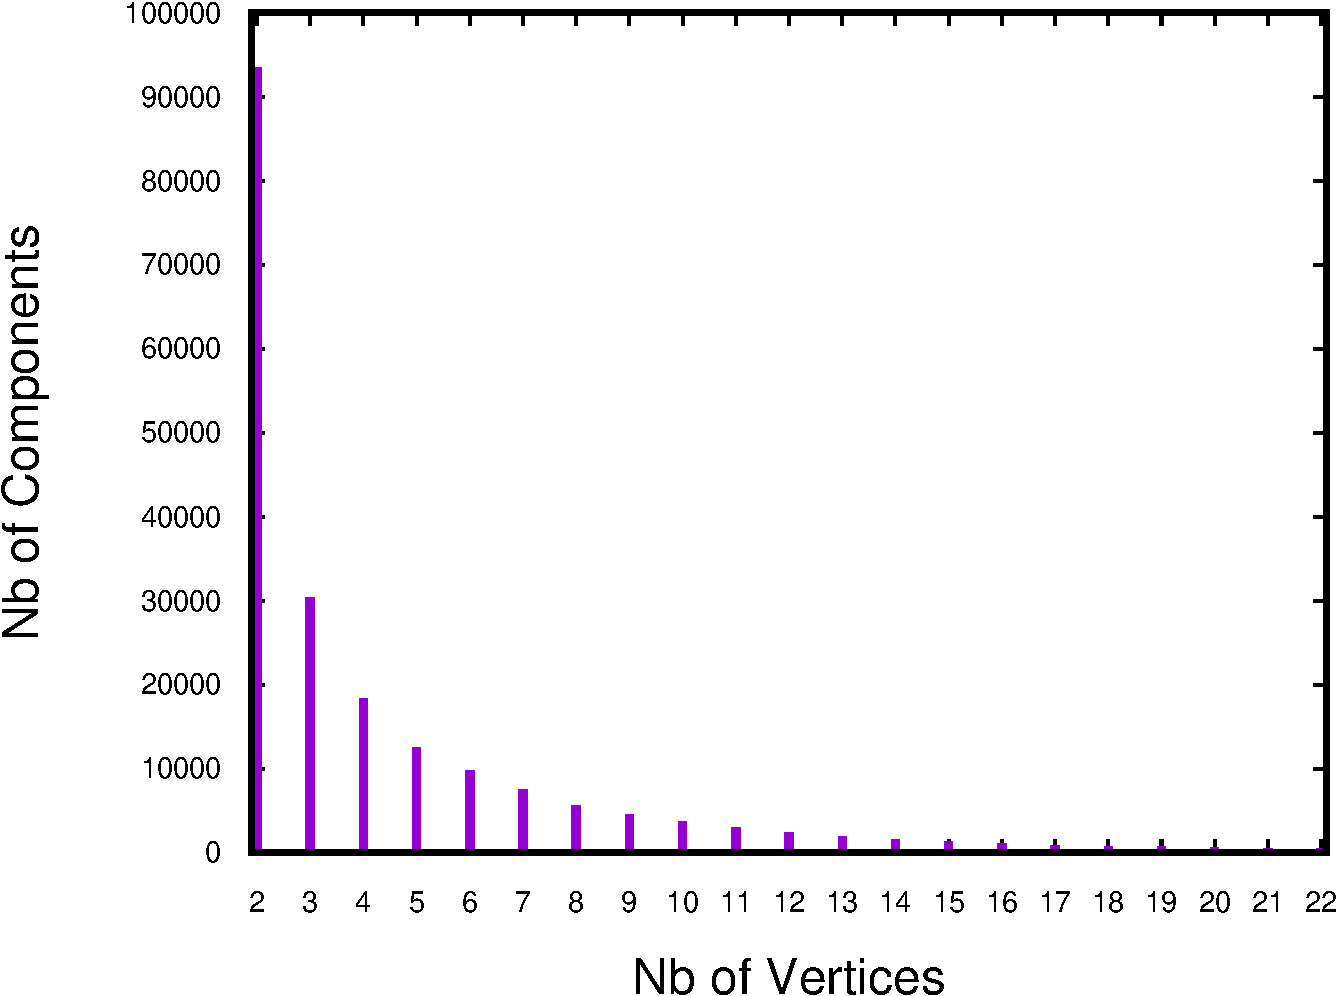
\includegraphics[scale=0.35]{bench/generated/frequency20-crop.pdf}
\caption{Distribution of components w.r.t. the number vertices (range from $2$ to $20$ vertices per component)}
\label{fig:vertices-components-20}
\end{figure}

\begin{figure}
\centering
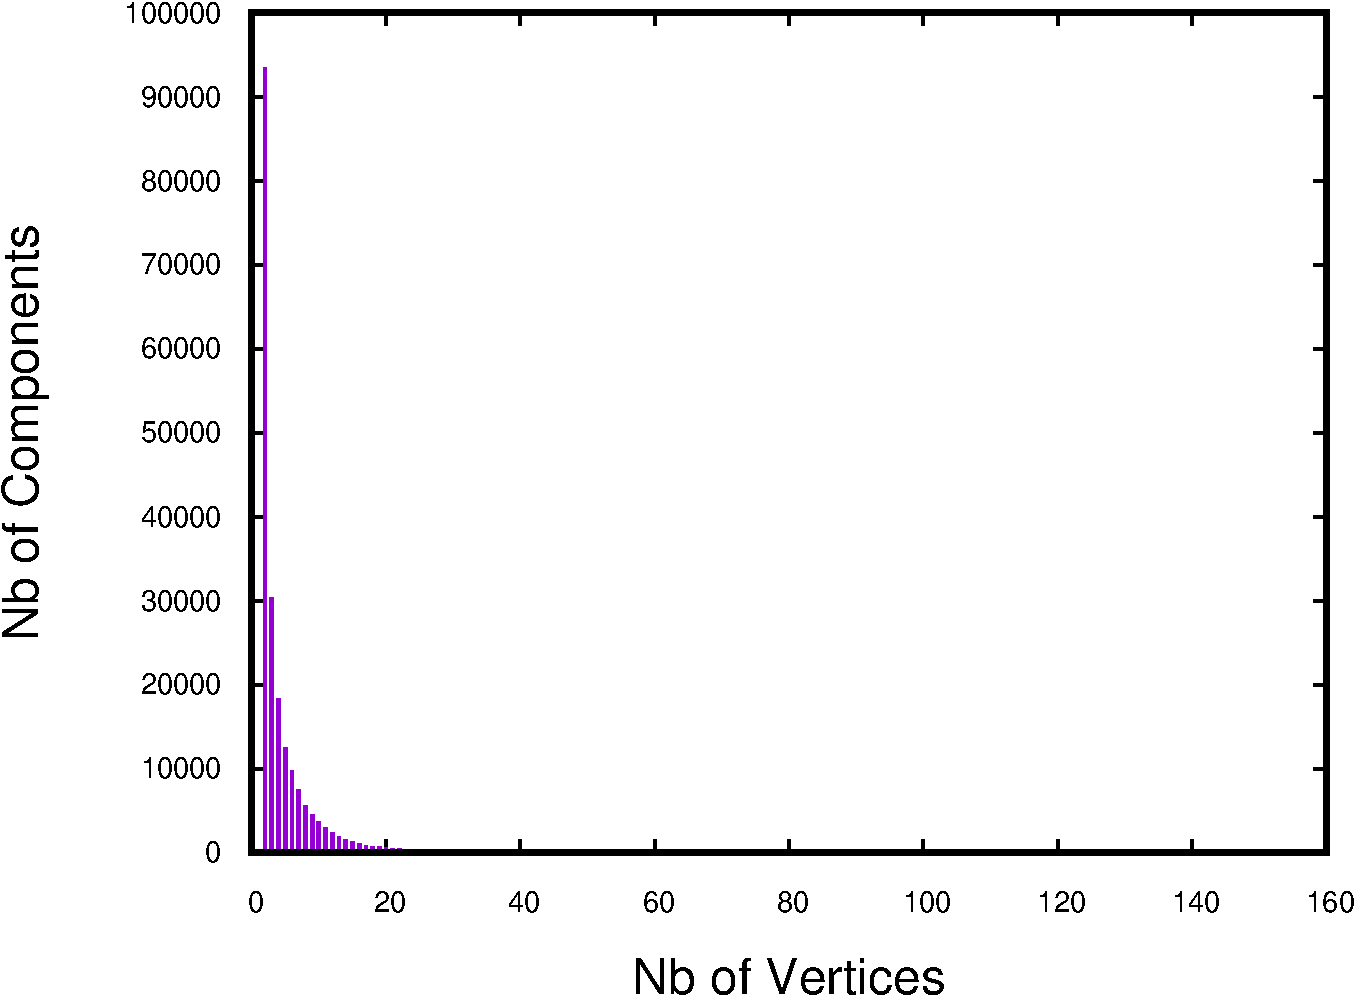
\includegraphics[scale=0.35]{bench/generated/frequencyall-crop.pdf}
\caption{Distribution of components w.r.t. the number vertices}
\label{fig:vertices-components-all}
\end{figure}

\begin{figure}
\centering
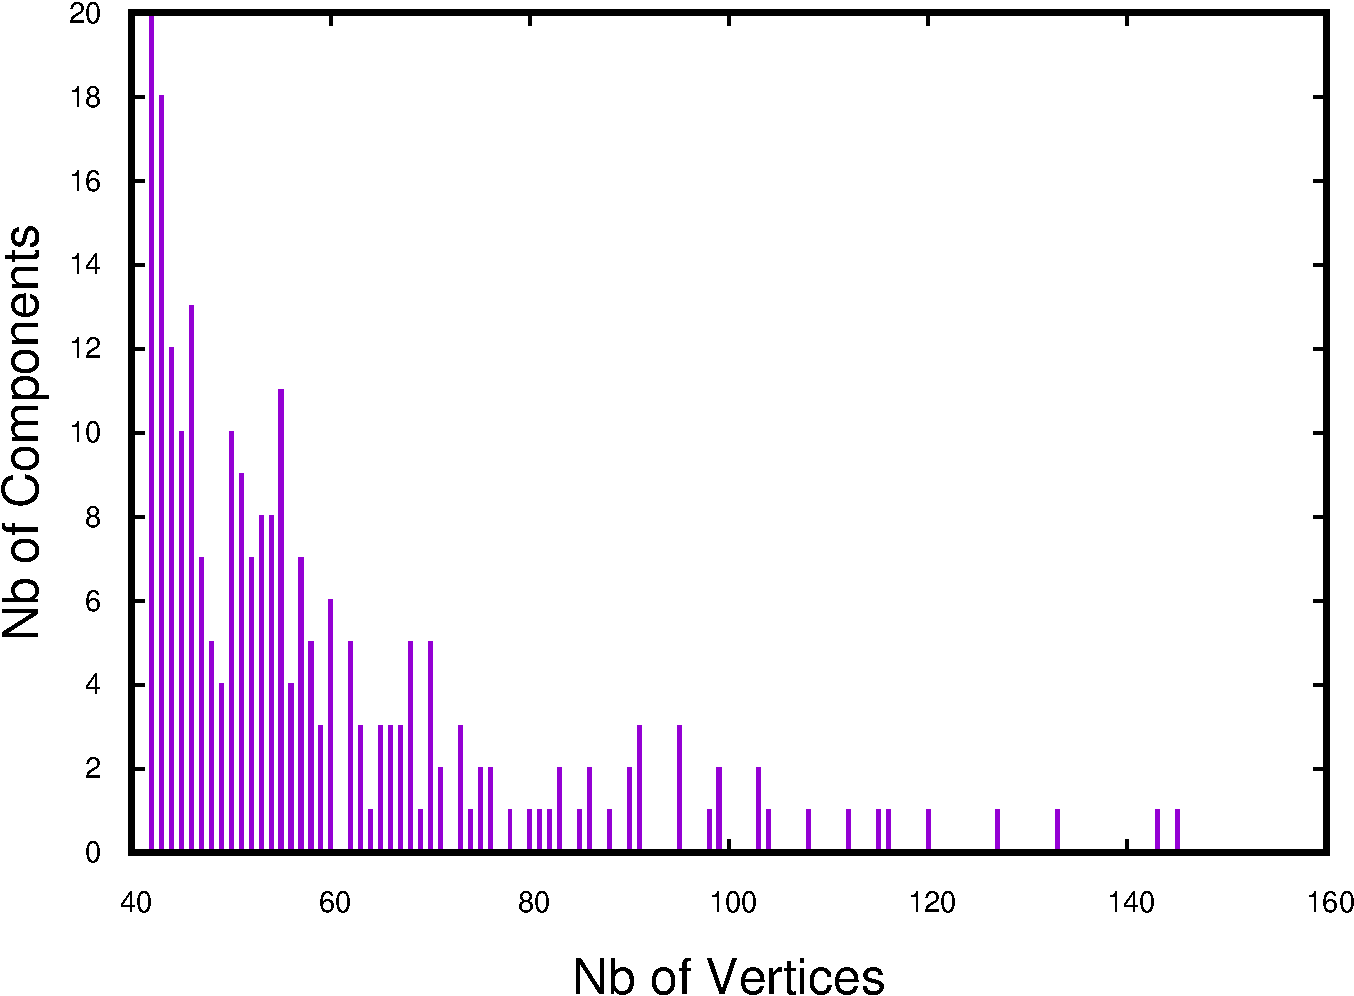
\includegraphics[scale=0.35]{bench/generated/frequency-selected-crop.pdf}
\caption{Distribution of components w.r.t. the number vertices (range from 40 to 140 vertices per component)}
\label{fig:vertices-components-40}
\end{figure}


% Because of this redundancy, the only way to achieve total failure is through the obvious choice of attacking all ten power plants. To exclude this obvious scenario from our contingency analysis, we remove all ten power plants from the associated graph model. This renders our contingency analysis completely focused on the irredundant nodes of the power grid. What remains are the high to medium step down stations that transform high voltage to medium voltage nodes as follows. As treated in \cite{2000Natur.406..378A}, a distribution substation is one that receives power from a single, high voltage transmission line, and distributes this on smaller voltage to consumers. However, when modeling the power grid here, we make no distinction between nodes representing transmission substations versus distributing substations. Since our distributed algorithm is aimed for big graphs, an exhaustive analysis of the power grid should be attempted, and as such, we preserve the power grid almost in its entirety with a few exceptions. 

\subsection{Random and Cascading Contingency Analysis}

Our baseline approach for navigating through node attacks follows that of \cite{2000Natur.406..378A}. A high level representation of the algorithm for implementing the random and cascading attacks is depicted in Algorithm~\ref{algo:random-cascading}. It captures both notions of node attack, followed by an evaluation of the loss in power flow capacity across the entire network.
%\begin{lstlisting}[language=java]
%attackGraph(Graph graph) {
%   for(i = 0 until |V|) {
%      select victim vertex v
%      remove vertex v
%      update loss with respect to v
%   }
%}
%\end{lstlisting}
%
\begin{algorithm}[ht]
\KwIn{Graph graph = (V, E)}
\KwOut{random and cascading attacks of the input graph}
    \SetKwFunction{FMain}{attackGraph}
    \SetKwProg{Fn}{Function}{:}{}
    \Fn{\FMain{graph}}{
        \For{$i \gets 0$ \KwTo $|V|$}
        {
        select victim vertex v\;
        remove vertex v\;
        update loss with respect to v\;
        }
}
\textbf{End Function}
 \caption{\edited{Random and cascading attacks}}
 \label{algo:random-cascading}
\end{algorithm}

Here, a victim vertex is chosen upon an examination of some measure of its centrality. Centrality is a quantitative measure that aims at revealing the importance of a node. Several indices of centrality tackled in the literature are based on geometric, spectral, as well as path-based measures. We refer the reader to \cite{BoldiVigna14} for a comprehensive survey. For undirected graphs, the geometric measure related to the indegree of a given node, as well as the path-based measure based on its betweenness, have both yielded a contextual understanding of connectivity loss in power grids (\cite{2000Natur.406..378A, JinAl10}). In line with this body of work, we select the victim vertex according to one of the following four scenarios:
\begin{itemize}
\item \emph{Random attacks}: a vertex is selected at random.
\item \emph{Attacks based on geometric centrality measure}: the vertex with the highest degree is selected. 
\item \emph{Attacks based on path-based centrality measure}: the vertex with the highest betweenness centrality is selected. The betweenness centrality of the nodes is only computed once (i.e., is not be updated after removing a vertex). 
\item \emph{Cascading attacks}: This is similar to the betweenness centrality scenario; however, the betweenness centrality of the nodes is updated at each iteration (i.e., after removal of a victim vertex).
\end{itemize}
Algorithm~\ref{algo:scenario-selection} depicts a more detailed snippet captures these four scenarios.
%\begin{lstlisting}[language=java]
%Compute betweenness centrality for each v in V
%
%attackGraph(Graph G = (V,E), bool Cascading) {
%   for(i = 0 until |V|) {
%      select victim vertex v in V
%      remove vertex v
%      if Cascading == TRUE
%         for each node not removed so far
%            recompute betweenness centrality
%      update loss with respect to v
%   }
%}
%\end{lstlisting}

\begin{algorithm}[ht]
\KwIn{Graph graph = (V, E), boolean cascading}
Compute betweenness centrality for each v in V\;
    \SetKwFunction{FMain}{attackGraph}
    \SetKwProg{Fn}{Function}{:}{}
    \Fn{\FMain{graph,  cascading}}{
        \For{$i \gets 0$ \KwTo $|V|$}
        {
         select victim vertex $v$ in $V$\;
               remove vertex $v$\;
        \If{$ cascading $}
            {
             \For{each node $u$ not removed so far}
             {
                 recompute betweenness centrality for $u$\;
             }
            }
      update loss with respect to $v$\;
        }
}
\textbf{End Function}
 \caption{\edited{Scenario-based victim selection}}
 \label{algo:scenario-selection}
\end{algorithm}

The choice behind node betweenness centrality is motivated by the following. Let $\sigma(s,t)$ denote the number of shortest paths between two vertices $s$ and $t$, and let $\sigma(s,t \left \vert \right. v)$ denote the number of shortest paths between $s$ and $t$ that pass through $v$. A most recent betweenness centrality (BC) score of $v$ is suggested by Brandes in \cite{Brandes01} as follows:
\begin{equation}
C(v) = \sum_{s,t \in V} \frac{\sigma(s,t \left \vert \right. v)}{\sigma(s,t)}
\label{brandesBC}
\end{equation}
where this assumes $s \neq t \neq v$, and considers $\sigma(s,s)=1$, $\sigma(s,t \left \vert \right. v)=0$ if $v = s$ or $v=t$, and $0/0 = 0$. With this definition, a high centrality score $C(v)$ implies that a vertex can reach others on relatively short paths, or that a vertex lies on a large number of shortest paths connecting other vertices. This particular choice of index is the basis for a quadratic running time, linear space algorithm by Brandes which improves on former cubic running time algorithms. The algorithm follows an accumulation technique that invokes a single-source shortest paths (SSSP) algorithm in multiple iterations starting from each vertex in the graph whose score needs to be produced. When the graph is unweighted, SSSP can be solved using breadth first traversals. To illustrate, let 
\begin{equation*}
\gamma(s, t \left \vert \right. v) = \frac{\sigma(s, t \left \vert \right. v)}{\sigma(s,t)}
\end{equation*}
denote the dependency of $s$ and $t$ on $v$, captured by the ratio of shortest paths between $s$ and $t$ that go through $v$. Also, let 
\begin{equation*}
\gamma(s \left \vert \right. v ) = \sum_{t \in V} \gamma(s,t \left \vert \right. v )
\end{equation*}
denote the dependency of $s$ on $v$, which is the sum of dependencies of $s$ and $t$ on $v$ for all possible targets $t$. 
We then have the following main result:
\begin{equation*}
\gamma(s \left \vert \right. v ) = \sum_{w: (v,w) \in E \land d(s,w) = d(s,v)+1} \frac{\sigma(s,v)\times (1+\gamma(s\left \vert \right. w))}{\sigma(s,w)}
\end{equation*}
where $d(s,w)$ is the shortest path length from $s$ to $w$ \cite{Brandes01}. The resulting algorithm now revolves around two steps:
\begin{enumerate}
\item For each $s \in V$, perform a breadth first traversal of the graph. In each traversal, compute the number of shortest paths from $s$ to all $t \in V$ going through a given other node $v \in V$. 
\item After each traversal, accumulate $\gamma (s,t \left \vert \right. v)$ into $\gamma(s \left \vert \right. v)$.
\end{enumerate}

\subsection{Connected Components: A localised view}
In contrast to the relatively smaller graphs treated in the literature on power grid resilience analysis, we have maintained the bulk of the power grid down to the finest spatial coordinates. Our graph with $\left \vert V \right \vert \approx 9 \times 10^6 $ represents a challenging size for serial computers and opportunities for distributed algorithm design ought to be explored. The fact that the high voltage power plants have been removed from the grid representation render the graph a disconnected one, consisting of 199004 connected components, where each component consists of transmission/distribution substations as nodes, and transmission lines between them as edges. Our Spark algorithm will distribute the work over these components, and for this, we begin by explaining the contextual implications of a decentralised version of the grid as such. This distribution of the network leads us to readdress the connectivity/loss and betweenness centrality in a manner that explores the effects of local changes on the global graph properties. We address those two issues separately below.

\subsubsection{Local versus global connectivity loss}
In \cite{2000Natur.406..378A}, the notion of loss manifests itself when less and less paths connect a power plant to a distribution station. In contrast, the Lebanese power grid has adapted to decades of power cuts that have resulted in a significant dependence on diesel power generators which, in theory, can connect to any transmission substation, say, within districts, or distribution substations, at the level of neighborhoods. These diesel generators are mobile and so their location may remain ``unknown'' to an attacker, and can be reasonably easily replaced. As such, the notion of loss in our scenario associates with attacks on transmission/distribution substations, and the removal of transmission lines between them, excluding the status of power plant generators or diesel generators. A node retains a power supply in the network so long as there exists a path of edges connecting it to any other node. Each time a victim vertex is attacked, all of its incident edges are removed along with it. As a result, we adopt the following definitions for connectivity and its loss. Given an undirected graph $G=(V,E)$, we define its connectivity as follows:
$$
\mathtt{connectivity}(G) = \sum_{v \in V} \mid \mathtt{reachable}(v) \mid,
$$
where $\mathtt{reachable}(v)$ is the set of all reachable nodes from $v$ via some path. 
This notion can be expanded as follows, where $G$ denotes an undirected graph:
\begin{equation}
\begin{array}{llr}
\mathtt{connectivity}(G) && \\
=  \mid V \mid \times \mid V-1 \mid & \mbox{if $G$ is connected,}& \\
 =  \sum_{i \in \{1,\ldots,n\}} \mathtt{connectivity}(G_i) & \mbox{otherwise.}&
\end{array}
\label{def}
\end{equation}
The following formula captures the percentage of loss as a result of attacking (removing) a node $x$ from $G$:
$$
\mathtt{loss}(G, x) = 1 - \frac{\mathtt{connectivity}(G \setminus \{x\})}{\mathtt{connectivity}(G)}
$$
where $G \setminus \{x\}$ is a graph defined by removing vertex $x$ in $G$ and all of its incident edges. For simplicity, we will track only the numerator appearing in this definition and consider hereafter that $\mathtt{loss}(G,x) = \mathtt{connectivity}(G)-\mathtt{connectivity}(G \setminus \{x\})$. The following proposition reveals how the local loss within a component translates to global loss:
\begin{proposition}
Let $G$ denote an undirected graph, and let $G_i$ denote the connected component to which $x$ belonged prior to its removal from $G$. We then have:
\begin{equation}
\begin{array}{ll}
\mathtt{connectivity}(G) - \mathtt{connectivity}(G \setminus \{x\}) &\\
= \mathtt{connectivity}(G_i) - \mathtt{connectivity}(G_i \setminus \{x\})
\end{array}
\label{loss}
\end{equation}
where $\mathtt{connectivity}(G_i \setminus \{x\})$ can be computed as in Eq. (\ref{def}) above.
\label{connectivity}
\end{proposition}
\begin{proof}
Since $G_i$ is a connected component of $G$ and $x \in G_i$, we have:
\begin{equation*}
\begin{array}{ll}
\mathtt{connectivity}(G \setminus \{x\})  &  \\
 =  \mathtt{connectivity}(G_i \setminus \{x\}) + \mathtt{connectivity}(G \setminus G_i)&\\
 =  \mathtt{connectivity}(G_i \setminus \{x\}) + \sum_{j = 1, j \neq i}^{n} \mathtt{connectivity}(G_j)&
\end{array}
\end{equation*}
We now use this equation in:
\begin{equation*}
\begin{array}{ll}
\mathtt{connectivity}(G) - \mathtt{connectivity}(G \setminus \{x\})  &  \\
 =  \sum_{j = 1}^{n} \mathtt{connectivity}(G_j) & \\
- \left ( \mathtt{connectivity}(G_i \setminus \{x\}) + \sum_{j = 1, j \neq i}^{n} \mathtt{connectivity}(G_j)\right)& \\
 =  \mathtt{connectivity}(G_i) - \mathtt{connectivity}(G_i \setminus \{x\}) 
\end{array}
\end{equation*}
\end{proof}
%%%%%%%%%%%%%%%%%%%%%%%%%%%%%%%%%%%%%%%%%%%%%%%%%%%%%%%%%%%%%%%%%%%%%%%%%%%%%%%%%%%%%%%%%%

\subsubsection{Local versus global centrality}

We now express the relationship between the global and local centrality measures for a given node within its connected component. We begin with the measure denoting the degree of a given vertex:
\begin{proposition}
Let $\mathtt{CC}(G) = \{G_1, \ldots, G_n\}$ denote the connected components of the undirected power grid graph $G$. Let $\deg_{G}(v)$ denote the degree of a node $v$ in $G$, and $\deg_{G_i}(v)$ denote its degree in $G_i$, for some connected component $G_i \in \mathtt{CC}(G)$ containing $v$. We then have:
\begin{equation*}
\deg_{G}(v) = \deg_{G_i}(v).
\end{equation*}
\label{degs}
\end{proposition}
\begin{proof}
The proof is straightforward: As $G$ is undirected, the edges incident on $v$ all belong to its connected component, and no edge outside its component can be incident on $v$.
\end{proof}
We now address the betweenness centrality measure: 
%Given a graph $G$, the betweeness centrality of a node $v$ is equal to $\mathtt{bc}_G(v) = \sum_{s \neq v \neq t} \frac{\sigma_{st}(v)}{\sigma_{st}}$, where $\sigma_{st}$ is the total number of shortest paths from node $s$ to node $t$ and $\sigma_{st}(v)$ is the number of those paths that pass through $v$. 
\begin{proposition}
Let $\mathtt{CC}(G) = \{G_1, \ldots, G_n\}$ denote the connected components of the undirected power grid graph $G$. Let $C_{G}(v)$ denote the BC score of a node $v$ in $G$, and $C_{G_i}(v)$ denote its BC score in $G_i$, for some connected component $G_i \in \mathtt{CC}(G)$ containing $v$. We then have:
\begin{equation*}
\mathtt{C}_{G}(v) = \mathtt{C}_{G_i}(v).
\end{equation*}
\label{BCs}
\end{proposition}
\begin{proof}
Let $s$, $t$, and $v$ denote distinct vertices in $V$. Since $G$ is undirected, we have $G_i \cap G_j = \emptyset$, $\forall i \neq j$. Hence, if $\exists i$ such that $s, t \in G_i$, then $\sigma(s,t)$, representing the number of paths between $s$ and $t$ in $G$, is identical to the number of paths between $s$ and $t$ in the subgraph $G_i$. Otherwise, $\sigma(s,t) = 0$. Similarly, if $\exists i$ such that $s, t, v \in G_i$, then $\sigma(s,t \left \vert \right. v)$, representing the number of paths between $s$ and $t$ in $G$ that pass through $v$, is identical to the number of paths between $s$ and $t$ in the subgraph $G_i$ that pass through $v$. Otherwise, $\sigma(s,t \left \vert \right. v) = 0$. Using Eq. \ref{brandesBC} for the BC score, we obtain that $\mathtt{C}_{G}(v) = \mathtt{C}_{G_i}(v)$ in all cases.
\end{proof}


\subsection{Spark-based Implementation}
We now present our Spark-based algorithm, guided by the propositions above. The many connected components of the power grid provide for an inherent data distribution of the graph which, as we will see in Sec. \ref{results}, allows for a balanced workload as well as locality of reference. Spark employs a storage abstraction called Resilient Distributed Datasets (RDDs). Each RDD is a distributed, fault-tolerant vector on which we can perform a set of vectorised operations. One can define a data partitioning scheme on a RDD. The execution engine can co-schedule tasks on those RDDs to avoid data movement. In what follows, we refer to threads that may be referenced within one single multithreaded machine or across several machines.
%
%Spark~\cite{spark} is new programming model supported by an execution engine for big data processing. Spark is based on RDD (Resilient Distributed Data Set). RDDs are big parallel collections that can be distributed across a cluster. RDDs are created through parallel transformations (e.g., map, group by, filter, join, create from file systems). Moreover, RDDs can be cached (in-memory) by allowing to keep data sets of interest in Memory across operations and thus contribute to a substantial speedup. At the same time, Spark uses lineage to support fault tolerance, i.e., record all the operations/transformations that yield to create RDDs from a source data. That is, in case of failure, an RDD can be reconstructed given the transformation functions yielding to that RDD. Additionally, after creating RDDs, it is possible to do analytics on them by running actions on them such as count, reduce, collect and save. Note that all operations/transformations are lazy until you run an action. Then, the Spark execution engine pipelines operations and finds an execution plan. GraphX~\cite{graphx} is a platform built on top of Spark that provides APIs for parallel and distributed processing on large graphs. 
%
\begin{enumerate}
\item Given a file (read from local or distributed file system, i.e., HDFS) containing information about the graph, build the corresponding graph RDD. Here, the input file is partitioned for distribution over the multiple threads. GraphX in Spark represents the graph internally as a pair of vertex and edge collections built on RDDs. 
\item Compute the connected components on the graph RDD using GraphX's built in strongly connected component distributed kernel. This creates an RDD, \texttt{rddCC}, of items, where each item corresponds to a connected component. 
\item Partition \texttt{rddCC} into several $p$ partitions, for $p = 4, \ldots, 32$, $p \leftarrow 2\times p$. Each partition is allocated to a single thread, and contains a number of connected components.  
\edited{
Note that, we use a customized partitioning scheme to get balanced partitions, i.e., large strongly connected components are spread among different partitions.}

\item The connected components within each partition are now distributed over the multiple threads on a single core (or multiple cores on a single thread). For each connected component, a thread $t$ selects a victim node according to one of the four scenarios, and locally updates the corresponding component by removing the victim vertex and its incident edges. Only the fourth scenario stipulates an update on the BC score of each remaining node. A tuple $(\rho,\lambda)$ is appended to the end of a list ${\bf L}_t$. Here, $\rho$ denotes its rank in the removal process if the vertex has been chosen in random order. Otherwise, $\rho$ denotes its centrality (degree or load based). Also, $\lambda$ denotes the loss percentage associated with the given victim node. 
\item Repeat Step 4 until all the nodes of a thread's connected component are identified. 
\item All threads now communicate their pairs in the list ${\bf L}_t$ to each other.
\item In the case where vertices have been removed in random order, define a reduce operation that concatenates the generated lists into a unified list ${\bf L}$. Else, define a reduce operation that merges all the generated lists on $b$ into ${\bf L}$. This step is performed serially.
\item Simulate the attack on $G$ by removing the nodes in ${\bf L}$ starting from the head. For each node $x_i$ removed from ${\bf L}$, return $loss(G,x_i) = \sum_{j = 1}^{i} \lambda_i$. This step is also performed serially.
\end{enumerate}
We now have the following:
\begin{proposition}
The above algorithm is correct, and returns $loss(G\setminus {\bf L})$, where ${\bf L}$ denotes the list of all nodes attacked in $G$.
\end{proposition}
\begin{proof}
We first address Step 4. By Prop. \ref{degs} and \ref{BCs}, each local measure of a centrality by one thread is also the global measure, and as such, computing it locally yields the answer independently of the other connected components within the same thread or on other threads. Also by a direct result of Prop. \ref{BCs}, updating the betweenness centrality scores after reach removal in the cascading scenario requires information about the paths connecting each vertex to vertices only in its own local component and thus can be performed independently of other threads. This allows to parallelise the computation of all betweeness centralities after attacking nodes in the cascading scenario. At the end of Step 4, the loss upon removal of each vertex is computed locally on each connected component item. By Prop. \ref{connectivity}, this local loss computed independently of other threads also indicates the global loss. 

We now address Step 7. If the scenario applied is the random hit scenario, concatenating the vertices from each thread violates no specific ordering on them, and thus one can proceed with the attacks as indicated by the concatenation. If the scenario applied relies on some measure of centrality, the merge procedure ensures that the locally ordered lists of vertices produced by each thread now yield a totally ordered sorted list on all the centrality measures, after which the attacks on nodes can begin to take place.

We conclude with Step 8. Write ${\bf L} = \{x_1,\ldots,x_n\}$, where $n = \left \vert L \right \vert$. Let $x$ and $y$ denote any two arbitrary nodes of $G$, and assume, without loss of generality, that $x$ was removed prior to $y$. Let $loss(G\setminus \{x,y\})$ denote the loss in the graph after removing $x$ followed by $y$. The losses returned in Step 7 are thus captured by $loss(G\setminus \{x_1,\ldots,x_n\})$:
\begin{itemize}
\item{Suppose that $x$ and $y$ do not belong to the same connected component. This can happen either when both of them are tackled by the same thread or otherwise. Whether or not the failures of $x$ and $y$ are happening simultaneously, the loss incumbent on removing $x$ is independent of the corresponding loss due to $y$, and so, $loss(G\setminus \{x,y\}) = loss (G \setminus \{x\}) + loss (G \setminus \{y\})$, i.e. the reduction operator on the individual losses can take place after the computation of individual losses locally in Step 4.}
\item{Otherwise, suppose that $x$ and $y$ belong to the same connected component. Then they certainly are tackled by the same thread. In this case, $x$ is failed before $y$ is failed, and so $loss(G\setminus \{x,y\})$ is computed correctly using the formula $loss(G \setminus \{x\}) + loss \left (\left(G \setminus \{x\}\right)\setminus \{y\}\right)$, which has already been computed locally in Step 4.} 
\end{itemize}
\end{proof}


\secondedited{We are now ready to conclude the analysis of our parallel design and we follow the exposition in \cite{Jordan02, Parhami99} to define the following terms. We call a parallel algorithm {\it work-optimal} if it has the smallest possible work, defined to be the smallest possible sequential work divided by the total number of processors. This excludes the cost of partitioning, which occurs at the beginning and thus is counted towards pre-processing costs, as well as the resulting data shuffling, which we regard as being memory or communication operations, not computation. We call a parallel algorithm {\it work-time-optimal}, if in addition to being work-optimal, its time is best possible. In the following proposition, we show that our resulting parallel design is work-optimal according to the definition above. However, due to partitioning and data shuffling costs, our algorithm fails to be work-time optimal.}

\begin{proposition}
The parallelised block in Steps 1--6 of the above algorithm maintains optimal parallel work, and requires linear time communication costs and a constant number of synchronisation barriers in the BSP model. Particularly, let $p$ denote the number of threads, $W_s$ denote the serial work of the algorithm in Steps 1--6, $g$ denote the machine-dependent cost in flops to communicate one data work, and $\ell$ denote the machine-dependent cost in flops for all threads to synchronise. We then have:
\[
T_p = \Theta\left(\frac{W_s}{p}\right) + \Theta \left(\frac{\left \vert V \right \vert}{p}\right) + 2 \ell \quad \mbox{flops.} 
\]
\end{proposition}
\begin{proof}
Here, we are addressing the costs of the parallelised block in Steps 1--6. In Steps 1 and 2, the data is distributed equally among all partitions, and within each partition, the Spark scheduler assigns available threads to the tasks required by Step 4. Let $W_s$ denote the serial work required by the algorithm in Steps 1--6. Because Step 4 engages all of the threads on the equally distributed data, its cost is accounted for by $\Theta\left(\frac{W_s}{p}\right)$. 
%
\edited{A parallel algorithm is work-optimal if it does not run more instructions than the sequential version and as such our algorithm is work-optimal.}
%
Step 6 is a communication step in which all threads in one partition communicate a pair of integers associated with each vertex they have been tasked with, and so, by the balanced data distribution of the earlier steps, the communication cost is $\Theta \left (g \cdot \frac{\left \vert V \right \vert}{p} \right)$ flops. The only synchronisation barriers needed are at the end of supersteps 1--4, and after the communication step in 6. This concludes the proof.
\end{proof}

\subsection{Spatial Correlation Analysis}

Here we study the spatial correlation between the targeted nodes in the cascading attacks scenario in an attempt to uncover any underlying spatial pattern. For this purpose, and using the geocoding of the input vertices, we examine the subset of nodes $F$ whose removal lead to a $90 \%$ connectivity loss. We are interested in measuring the the relation between failures separated by some given distance $r$. Following closely the spatial analysis of the 1996 blackout of Western Systems Coordinating Council area conducted in \cite{DaqingAl14}, we adopt the spatial correlation function $C(r)$ that measures the relation between failures that are $r$ distance apart:
\begin{equation}
C(x) \propto \frac{\sum_{{ij}\in F} (x_i- \bar{x} )(x_j - \bar{x}) \delta(r_{ij} - r)}{\sum_{ij \in F} \delta (r_{ij} - r)},
\end{equation}
Here, $x_i=1$ if node is is failed, and $0$ otherwise. Also, $\bar{x}$ denotes the average number of cascading failures over the whole network, $\delta$ denotes the function that singles out the $j$ nodes that are $r$ distance apart from $i$, and $r_{ij}$ denotes the Euclidean distance between nodes $i$ and $j$. Positive values for $C(r)$ indicate a tendency of failures to be close to each other, while negative values indicate anti-correlations.  



%%% end